\section{Модель}\label{sec:model}

Существующие решения, показывающие наилучшие результаты на опубликованных датасетах для Java \cite{Yang2017} и C++ \cite{Caliskan2015}, используют факторы, специфичные для конкретных языков. В этой работе предлагается два решения, основывающиеся на представлении кода при помощи контекстов в AST \cite{Alon2018}, работающие с произвольным языком программирования. Модели предназначены для работы с разным количества примеров, доступных для каждого автора. Первая модель применима при числе примеров порядка тысячи и более, вторая — при числе примеров в пределах нескольких сотен.

\subsection{Модель на основе code2vec}

Схема работы метода векторизации кода на основе контекстов в AST представлена на Рис. \ref{fig:code2vec-original}. В дереве выделяются листья и соответствующие им токены. Они нумеруются в порядке появления в коде. Затем из дерева выделяются тройки из пары токенов и пути между ними, называемые контекстами. Токены называются начальным и конечным в порядке их появления в коде. Путь представляет из себя последовательность типов вершин в порядке от начального листа до конечного и пометок о том, вверх или вниз совершен переход. На Рис. \ref{fig:ast-example} приведен пример AST, построенного по фрагменту кода. Цветом выделен путь между двумя листьями. Этому пути соответствует следующая последовательность, где стрелками обозначается направление перехода между вершинами, а типы сокращаются по первым буквам:
$$SN \uparrow MD \downarrow B \downarrow RS \downarrow IE \downarrow SN$$

Контекст, образованный из пути и токенов на его концах выглядит следующим образом:
$$(square, SN \uparrow MD \downarrow B \downarrow RS \downarrow IE \downarrow SN, x)$$

Фрагмент кода представляется мультимножеством контекстов, содержащихся в его AST. Если фрагмент содержит $N$ токенов, то размер мультимножества будет равен количеству пар токенов и асимптотически равен $O(N^2)$. Чтобы уменьшить их количество, вводится ограничение на разницу в индексах между начальным и конечным токеном, называющуюся шириной, и количество вершин в пути, называющееся длиной. Если ширина ограничена значением $w$, то контекстов останется $O(Nw)$.

\begin{figure}[ht]
    \centering
       \begin{subfigure}{0.35\linewidth}
       \centering
       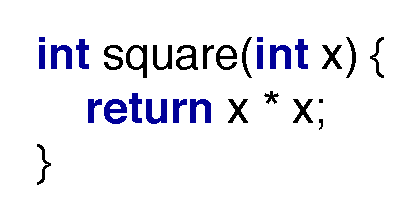
\includegraphics[width=\linewidth]{images/AstCode.pdf}
       \caption{}
       \label{fig:ast-code} 
    \end{subfigure}
    \\[\baselineskip]
    \begin{subfigure}{0.98\linewidth}
       \centering
       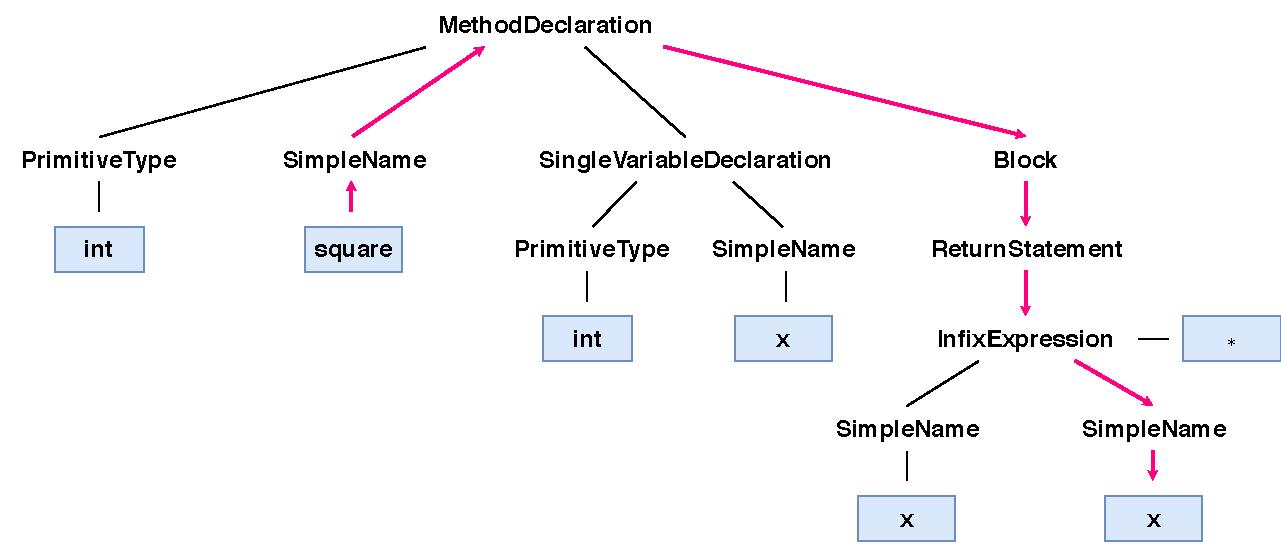
\includegraphics[width=\linewidth]{images/AstExample.pdf}
       \caption{}
       \label{fig:ast-example}
    \end{subfigure}
    \centering
    \caption{(a) Пример фрагмента кода. (b) AST, построенное по фрагменту кода при помощи библиотеки GumTree \cite{GumTree}. Цветом выделен путь между парой листьев.}
    \end{figure}

Каждому пути и токену сопоставляется вектор эмбеддинга. Эмбеддинг — это обучаемое отображение из конечного множества в векторное пространство. Изначально оно выбирается случайным, а в процессе обучения модели модифицируется. Контексту сопоставляется конкатенация из трёх векторов, соответствующих токенам и пути. Затем, чтобы получить вектор для фрагмента кода, векторизации его контекстов складываются с весами, которые им назначает механизм внимания. Он реализуется при помощи скалярного произведения вектора контекста на вектор внимания, обучаемый вместе с моделью.

В данной работе модель была дополнена путём добавления возможности работать с группами из нескольких фрагментов кода. Ими могут быть методы, относящиеся к одному коммиту или находящиеся в одном файле, случайная выборка из всего множества методов, методы, написанные в определенный промежуток времени. Для этого в неё был добавлен ещё один слой с механизмом внимания, агрегирующий векторизации нескольких фрагментов в одну. Помимо увеличения точности модели он позволяет выделить фрагменты, имеющие большее значение при решении задачи, в нашем случае — при определении авторства группы из нескольких методов. Модифицированная архитектура представлена на Рис. \ref{fig:code2vec-enhanced}.

    \begin{figure}[ht]
    \centering
       \begin{subfigure}{0.98\linewidth}
       \centering
       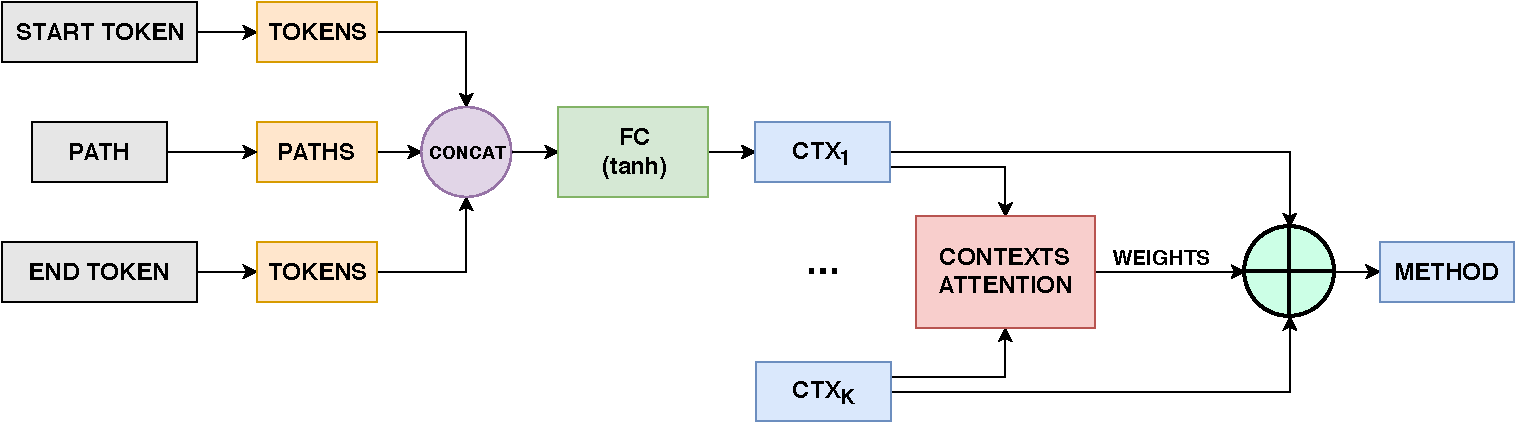
\includegraphics[width=\linewidth]{images/Code2VecOriginal.pdf}
       \caption{}
       \label{fig:code2vec-original} 
    \end{subfigure}
    \\[\baselineskip]
    \begin{subfigure}{0.34\linewidth}
       \centering
       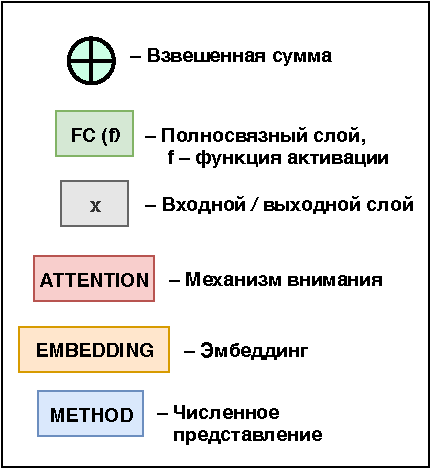
\includegraphics[width=\linewidth]{images/Code2VecLegend.pdf}
       \caption{}
       \label{fig:code2vec-legend}
    \end{subfigure}
    \hfill
    \begin{subfigure}{0.54\linewidth}
       \centering
       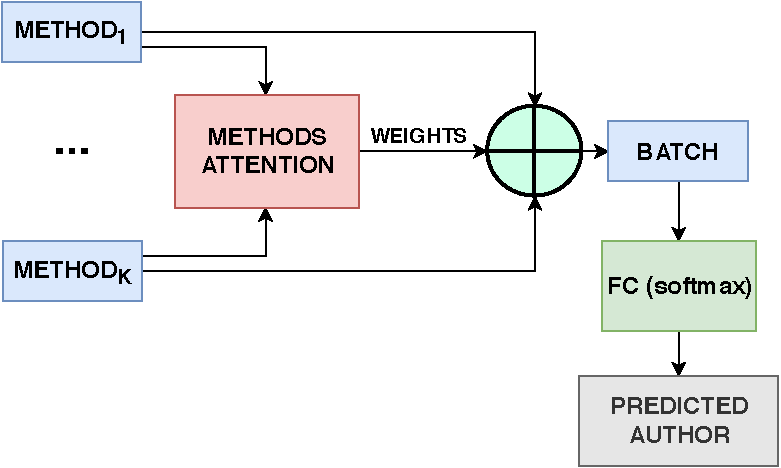
\includegraphics[width=\linewidth]{images/Code2VecEnhanced.pdf}
       \caption{}
       \label{fig:code2vec-enhanced}
    \end{subfigure}
    \centering
    \caption{(a) Архитектура модели code2vec \cite{Alon2019}. (b) Условные обозначения для описания нейросетевой архитектуры. (c) Расширение архитектуры code2vec для работы с группами из нескольких методов.}
    \end{figure}

Количество параметров в предложенной модели зависит от числа различных путей и токенов и от размерности используемых векторных представлений. Обозначим число параметров за $ModelSize$ и запишем его асимптотику:
$$ModelSize = O(Td+Pd),$$
где $T$ — число токенов, $P$ — число путей, $d$ — размерность векторизаций.

Число различных путей и токенов для датасетов, использованных в предыдущих работах, а также количество примеров, доступных для обучения, приведено в таблице \ref{tab:datasets-sizes}. Количество параметров модели даже при выборе значения размерности равного 1 остается на порядок выше, чем число примеров, поэтому для наборов данных с высоким соотношением числа различных токенов и путей к размеру датасета предлагается вторая модель.

Модель может применяться для любого языка программирования, по коду которого можно построить AST. Таковыми является большинство популярных языков программирования, так как в них AST используется компиляторами и интерпретаторами для промежуточного представления кода. Для построения AST и дальнейшего получения контекстов используется библиотека, более подробно описанная в разделе \ref{sec:data}.

\vskip 1em
	\begin{table}[ht]
      \caption{Размеры датасетов, использовавшихся в предыдущих работах и число различных токенов и путей, встречающихся в них. Приведено число различных путей с шириной не более 3 и длиной не более 10.}
		\centering
      \begin{tabular}{|c|c|c|c|}
         \hline
                                           & \textbf{C++} & \textbf{Java} & \textbf{Python} \\ \hline
         \textbf{Число авторов}            & 1600         & 40            & 70              \\ \hline
         \textbf{Размер датасета (файлов)} & 14400        & 3021          & 700             \\ \hline
         \textbf{Различные токены (тыс.)}  & 30.2         & 36.7          & 4.3             \\ \hline
         \textbf{Различные пути (тыс.)}    & 169.9        & 7.9           & 46.3            \\ \hline
         \textbf{Токены и пути / Размер}   & 13.9         & 14.8          & 72.3            \\ \hline
      \end{tabular}
		\label{tab:datasets-sizes}
   \end{table}
   
\subsection{Модель на основе случайного леса}

Вторая модель представляет из себя случайный лес. В качестве факторов используются те же данные, которые образовывали контексты, описанные выше: частоты встречаемости путей между листьями в AST и частоты встречаемости токенов на их концах. Таким образом, каждый фрагмент кода представляется разреженным вектором размера $P+2T$. Для работы модели, как и в предыдущем случае, требуется построение AST, что возможно для большинства современных языков программирования.

Для улучшения качества работы модели применяется фильтрация множества факторов при помощи подсчета совместной информации между значением фактора и автором фрагмента. Совместная информация двух случайных величин определяется следующим образом:
$$I(A;F) = H(A) + H(F) - H(A, F),$$
где $A$ — множество авторов, $F$ — множество факторов, $H(X)$, $H(Y)$, $H(X,Y)$ — энтропия и условная энтропия случайных величин.

В результате фильтрации остаются только факторы с высоким значением совместной информации с целевой функцией. Доля факторов, которая остается после фильтрации, определяется эмпирически. Полученные эмпирические значения, результаты применения модели на различных датасетах, сравнение моделей между собой и с существующими решениями приведено в главе \ref{sec:evaluation}.

У модели есть два гиперпараметра: число деревьев в лесу и количество факторов, остающихся после фильтрации. Для их подбора применяется кросс-валидация и поиск по сетке. Качество работы модели оценивается путем кросс-валидации, перебирая разные значения гиперпараметров, и эмпирически устанавливаются оптимальные значения. Они варьируются в зависимости от набора данных: оптимальная доля остающихся после фильтрации факторов составляет от 5\% до 10\%, а оптимальное число деревьев — от 300 до 500.

\subsection{Выводы}
Эта работа предлагает две модели для определения авторства в условиях разного количества данных. В обоих случаях по фрагменту кода строится AST, а затем он представляется в виде набора контекстов, состоящих из путей между парами листьев в AST и токенами на их концах. Первая из моделей — нейронная сеть, использующая механизм внимания для получения векторного представления фрагмента кода из эмбеддингов путей и токенов. Ее целесообразно использовать, когда количество различных путей и токенов сопоставимо или меньше числа доступных для обучения примеров, на практике это тысячи или десятки тысяч примеров для каждого автора. Вторая модель — случайный лес из 500 деревьев, строящийся по частотам встречаемости токенов и путей, встречающихся в фрагменте кода. Для фильтрации множества факторов применяется метод фильтрации на основании совместной информации значения фактора и автора кода. Случайный лес целесообразно использовать, когда размер датасета меньше, чем число различных путей и токенов.
